\begin{figure}
    \centering
\begin{knitrout}
\definecolor{shadecolor}{rgb}{0.969, 0.969, 0.969}\color{fgcolor}
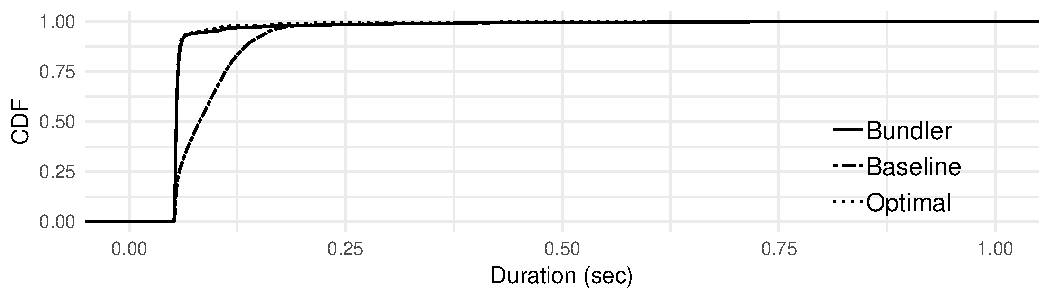
\includegraphics[width=\maxwidth]{figure/eval:best-1} 

\end{knitrout}
    \caption{\name achieves 33\% lower median slowdown. Note the differing axis scales. For both \name and Optimal, performance benefits come from preventing short flows from queueing behind long ones.}
    \label{fig:eval:best}
\end{figure}
\newcommand{\overviewBenefitsBaselineMedian}{1.62}
\newcommand{\overviewBenefitsBaselineTail}{10.77}
\newcommand{\overviewBenefitsBundlerMedian}{1.08}
\newcommand{\overviewBenefitsBundlerTail}{9.84}
\newcommand{\overviewBenefitsOptimalMedian}{1.08}
\newcommand{\overviewBenefitsOptimalTail}{4.46}
\newcommand{\overviewBenefitsBundlerMedianImprovement}{33.25\%}
